\documentclass[a4paper, 12pt]{article}
\usepackage[a4paper,top=1.5cm, bottom=1.5cm, left=1cm, right=1cm]{geometry}

% Работа с русским языком
\usepackage[utf8]{inputenc}
\usepackage{mathtext}                % русские буквы в формулах
\usepackage[english, russian]{babel} % локализация и переносы

\usepackage{graphicx}   % Вставка изображений
\usepackage{float}      % "Плавающие" изображения
\usepackage{wrapfig}    % Обтекание фигур (таблиц, картинок и прочего)
\graphicspath{ {./images/} }

\usepackage{multirow}
\usepackage{amsmath}
\usepackage{amsfonts}
\usepackage{indentfirst}
\usepackage{longtable}
\graphicspath{{pictures/}}
\usepackage{natbib}


\title{Работа 2.3.1 \\ Получение и измерение вакуума}
\author{Дмитрий Тихонов, ФРКТ, Б01-206}
\date{15 февраля 2023 г.}

\begin{document}
	\maketitle

    \section*{Введение}
        \subsection*{Цель работы:} изучение принципов получения и измерения вакуума в экспериментальном стенде на основе компактного безмасляного высоковакуумного откачного поста, вакууметров.
        \subsection*{В работе используются:} турбомолекулярный насос HiPace 80, форвакуумный насос MVP 015, комбинированный вакуумметр MPT 100 (В2) типов Пирани (терморезисторный) и холодный катод (инвертированный магнетрон).
        
    \section*{Теоретические сведения}
        Одна из основных характеристик систем, работающих при вакууме -- число Кнудсена:

        \begin{equation}
            Kn = \frac{\lambda}{d}, 
        \end{equation}
        где $\lambda$ -- длина свободного пробега молекул газа, $d$ -- характерный размер системы.

        В зависимости от значений числа Кнудсена определяют:
        \begin{itemize}
            \item низкий вакуум -- $Kn \ll 1$
            \item средний вакуум -- $Kn \sim 1$
            \item высокий вакуум -- $Kn \gg 1$
        \end{itemize}

        Выделим основные формулы, отображающие теоретические зависимости между исследуемыми величинами.

        Скорость откачки:
        \begin{equation}
            S = \frac{dV}{dt};
        \end{equation}	

        Падение давления:
        \begin{equation}
            \Delta P = P_{\text{вх}} - P_{\text{вых}};
        \end{equation}

        Пропускная способность:
        \begin{equation}
            U = \frac{Q}{\Delta P};
        \end{equation}

        Основное уравнение вакуумной механики:
        \begin{equation}
            \frac{1}{S_{0}} = \frac{1}{S_{\text{н}}} + \frac{1}{U};
        \end{equation} 

        \begin{equation}
            Q_{\text{н}} = V\frac{P_{\text{к}} - P_{\text{н}}}{\Delta t}		
        \end{equation}

        Проводимость отверстия:
        \begin{equation}
            U_{\text{отв}} = \frac{1}{4} \pi R^{2} \sqrt{\frac{8kT}{\pi m}} \sim R^{2}\sqrt{T/m}
        \end{equation}

        Проводимость длинного трубопровода
        \begin{equation}
            U_{\text{тр}} = \frac{4}{3} \frac{R^{3}}{L} \sqrt{\frac{2\pi kT}{m}} \sim \frac{R^{3}}{L} \sqrt{\frac{T}{m}} 
        \end{equation}

        Уравнение откачки газа
        \begin{equation}
            P\left( t \right) = P_{1}\exp \left(- \frac{S_{0}}{V_{0}}t \right)
        \end{equation}
            
    \section*{Методика измерений и используемое оборудование}
        \begin{figure}[H]
            \centering
            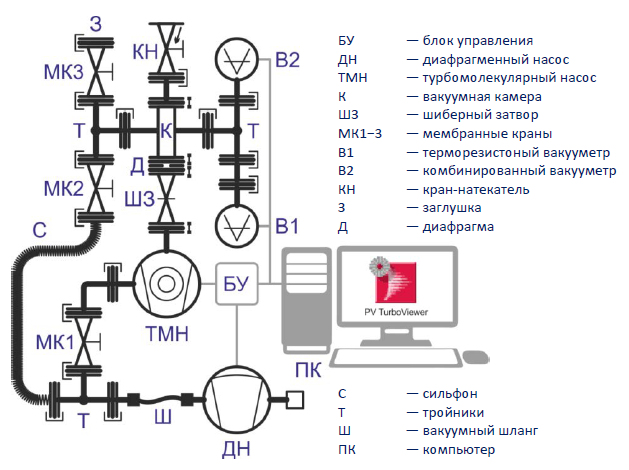
\includegraphics[width = \textwidth]{images/231_1.png}
            \caption{Схема экпериментальной установки}
        \end{figure}
        
        Экспериментальный стенд выполнен на основе компактного безмасляного высоковакуумного откачного поста Pfeiffer Vacuum серии HiCube 80 Eco с диафрагменным и турбомолекулярным насосами, вакуумметров Pfeiffer Vacuum серии DigiLine, и вакуумных быстроразъёмных компонентов. Управление основными функциями откачного поста, контроль и запись параметров установки осуществляется блоком управления (БУ) через цифровой интерфейс RS-485 с помощью специального программного обеспечения PV TurboViewer8.
        Вакуумный пост Pfeiffer Vacuum HiCube 80 Eco (PM S03 555 А) выполнен на базе диафрагменного форвакуумного насоса MVP 015 (ДН) и турбомолекулярного насоса HiPace 80 (ТМН). Откачка вакуумной камеры (К) может происходить как двумя насосами (ТМН и ДН) через шиберный затвор (ШЗ) и мембранный кран 1 (МК1), так и только форвакуумным насосом (ДН) по схеме «байпас» (англ. bypass — обходной путь), выполненной на основе вакуумных компонентов: сильфона (С), мембранного крана 2 (МК2), тройников (Т), переходников, шланга (Ш). Для контроля и измерения давления в вакуумной камере используются цифровой вакууметр PPT 100 (В1) типа Пирани (терморезисторный) и комбинированный вакуумметр MPT 100 (В2) типов Пирани (терморезисторный) и холодный катод (инвертированный магнетрон). Контролированный напуск воздушной атмосферы в камеру осуществляется через кран-натекатель EVN 116 (КН) с регулируемым потоком. Дополнительный выход с краном 3 (МК3) закрыт заглушкой (З) и служит для присоединения дополнительного объёма в случае необходимости.

        \begin{figure}[H]
            \centering
            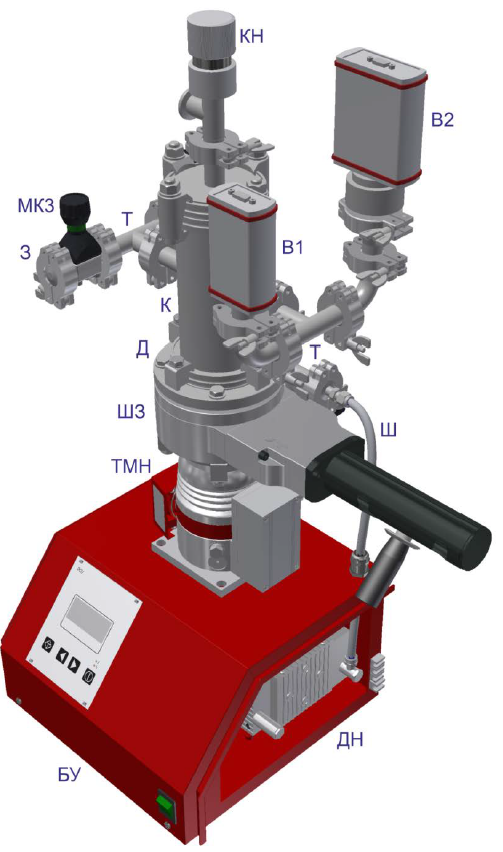
\includegraphics[scale = 0.8]{images/231_2.png}
            \caption{Схема экпериментальной установки}
        \end{figure}
        
    
    \section*{Результаты измерений и обработка данных}
        \subsection*{Определение откачиваемого объёма}
        Для определения объемов частей установки (объём вакуумной камеры -- $V_{K}$, объём форвакуумной магистрали и объём турбомолекулярного насоса -- $V_{\text{ф.м. + тмн}}$) воспользуемся законом Бойля-Мариотта. Для этого необходимо определить давления в различных частях установки. Результаты измерений были занесены в таблицу \ref{tab:results_of_measuring_for_value}.
	
        \begin{table}[H]
            \centering
            \begin{tabular}{|c|c|c|c|}
                \hline
                $p_{атм}, мбар$ & $p_1, мбар$ & $p_2, мбар$ & $p_3, мбар$ \\ \hline
                1000.0 & 5.1 & 280.0 & 170.0 \\ \hline
            \end{tabular}
            \caption{Результаты измерения давления при различных конфигурациях системы.}
            \label{tab:results_of_measuring_for_value}
        \end{table}

        Используя закон Бойля-Мариотта и зная, что $V_{\text{сильф}} = 265 \: \text{мл}$ получаем соотношения:
	
        \begin{equation}
            V_{K} = \frac{p_{\text{атм}} - p_{2}}{p_{2} - p_{1}}V_{\text{сильф}} = 694 \: \text{мл}
            \label{eq:value_of_vacuum_cam}
        \end{equation}
	
	\begin{equation}
            V_{\text{ф.м. + тмн}} = \frac{ \left( p_{3} - p_{2}\right)\left(V_{K} + V_{\text{сильф}}\right) }{p_{1} - p_{3}} = 640 \: \text{мл}
		\label{eq:value_of_forvacuum_tube}
	\end{equation}

        Отсюда, полный объём установки:
        $$
        \boxed{V_0 = V_{K} + V_{\text{ф.м. + тмн}} = 1334 \text{мл}}
        $$
 
        \subsection*{Измерение скорости откачки форвакуумным насосом}
            Рассмотрим откачку установки форвакуумным насосом. Построим график зависимости давления от времени (рис. \ref{graph:forvakuum}, рис. \ref{graph:approx_forvakuum}).

            \begin{figure}[H]
                \centering
                \includegraphics[width = \textwidth]{images/lnP(t)_forvakuum.png}
                \caption{Зависимость давления от времени для откачки форвакуумным насосом}
                \label{graph:forvakuum}
            \end{figure}
            
            \begin{figure}[H]
                \centering
                \includegraphics[width = \textwidth]{images/approx_lnP(t).png}
                \caption{Зависимость давления от времени для откачки форвакуумным насосом (касательная)}
                \label{graph:approx_forvakuum}
            \end{figure}

            Характеристики откачки можно получить по основному уравнению вакуумной техники:
            \begin{equation}
                \frac{1}{S_0} = \frac{1}{S_H}+\frac{1}{U} 
            \end{equation}
            
            \begin{table}[H]   
                \centering
                \begin{tabular}{|c|c|c|c|}
                    \hline 
                    $\tau$, c & $S_0$, мл/с& $S_H$, мл/с& U, мл/с  \\ 
                    \hline 
                    17.0 $\pm$ 0.5 & 78 $\pm$ 3 & 140 & 176 $\pm$ 7\\ 
                    \hline  
                \end{tabular} 
                \caption{Характеристики откачки форвакуумным насосом}
            \end{table}

        \subsection*{Измерение скорости откачки турбомолекулярным насосом}
            Рассмотрим откачку установки турбомолекулярным насосом. Построим график зависимости давления от времени (рис. \ref{graph:turbo}, рис. \ref{graph:approx_turbo}).

            \begin{figure}[H]
                \centering
                \includegraphics[width = \textwidth]{images/lnP(t)_turbomol.png}
                \caption{Зависимость давления от времени для откачки турбомолекулярным насосом}
                \label{graph:turbo}
            \end{figure}
            
            \begin{figure}[H]
                \centering
                \includegraphics[width = \textwidth]{images/approx_lnP(t)_turbo.png}
                \caption{Зависимость давления от времени для откачки турбомолекулярным насосом (касательная)}
                \label{graph:approx_turbo}
            \end{figure}

            Характеристики откачки можно получить по основному уравнению вакуумной техники:
            \begin{equation}
                \frac{1}{S_0} = \frac{1}{S_H}+\frac{1}{U} 
            \end{equation}
            
            \begin{table}[H]   
                \centering
                \begin{tabular}{|c|c|c|c|}
                    \hline 
                    $\tau$, c & $S_0$, мл/с& $S_H$, мл/с& U, мл/с  \\ 
                    \hline 
                    33 $\pm$ 1 & 42 $\pm$ 2 & 60000 & 42 $\pm$ 2\\ 
                    \hline  
                \end{tabular} 
                \caption{Характеристики откачки турбомолекулярным насосом}
            \end{table}

        \subsection*{Оценка уровней течей}
        Найдем натекание при закрытии насоса шлюзом, используя значения давления в эти моменты.
        
        \begin{equation}
            Q_H = V\frac{P_K-P_H}{\Delta t} \approx 10^{-5} \text{Дж/с}
        \end{equation}
        
        Проверим допустимость натекания:
        \begin{equation}
            10^{-7} \text{Дж/с} = Q_H \ll Q = P_1 S_0 = 10^{-2} \text{Дж/с}
        \end{equation}
        
        Вследствие этого неравенства натекание в системе можно считать допустимым.

        \subsection*{Исследование зависимости мощности турбины насоса от давления в камере}

        Построим график зависимости $p(W)$ в диапазоне предельных давлений. Данный график изображен на рис. \ref{fig:Depence_preasure_of_power}.
        
        \begin{figure}[H]
            \begin{center}
            \includegraphics[width = 0.95\textwidth]{images/W(P).png}
            \caption{График зависимости $W$ от $P$}
            \label{fig:Depence_preasure_of_power}
            \end{center}
        \end{figure}
        
        Как видно из графика, полученная зависимость имеет линейный характер с характерным переходным процессом. Данный переходный процесс можно считать моментом перехода в молекулярный режим течения газа.
        
        Давление, при котором происходит переход в молекулярный режим течения: $\sim 1,5 \cdot 10^{-3} \: мбар$ при данном давлении мощность турбины насоса составляла 27-28 Вт. Наглядно просматривается зависимость эффективности работы турбомолекулярного насоса от предельного давления в камере насоса.

        График $W(P)$ имеет вид линейной зависимости исходя из основного уравнения вакуумной механики и формулы ля проводимости длинного трубопровода.
	
        \subsection*{Оценка числа Кнудсена для предельных давлений}
            Рассчитаем число Кнудсена для предельных давлений по формуле:
            
            \begin{equation}
                Kn=\frac{\lambda}{d}=\frac{1}{\sqrt{2}nd\sigma}=\frac{kT}{\sqrt{2}d\sigma p}
            \end{equation}
            где $\sigma = 4.3 \cdot 10^{-19} {\text{{ м}}^2}$. Тогда получим следующие значения для числа Кнудсена (считая диаметр магистрали порядка 1 см):

            \begin{table}[H]
                \label{кнудсен}
                \centering
                \begin{tabular}{|c|c|c|}
                \hline 
                Часть установки & $P, мбар$ & $Kn$  \\ 
                \hline 
                Форвакуумная магистраль &  5.2 & $1.3\cdot 10^{-3}$ \\ 
                \hline 
                Форвакуумная магистраль & $1.5 \cdot 10^{-4}$  & 50\\ 
                \hline
                \end{tabular} 
                \caption{Число Кнудсена для предельных давлений}
            \end{table}

            Откуда получаем, что после откачки турбомолекулярным насосом число Кнудсена $Kn\gg 1$, что свидетельствует о молекулярном (кнудсеновском) режиме течения газа.    
    
    \section*{Заключение}

    \begin{itemize}
        \item в результате проведения эксперимента было выявлено, что установка работает корректно, то есть натеканием воздуха можно пренебречь при выполнении условий проведения опыта;

        \item было найдено давление, при котором наступает молекулярный режим течения газа (воздуха); 

        \item был вычислен коэффициент Кнудсена, который доказал применимость полученных теоретических формул;
        
        \item подтверждено большинство теоретических зависимостей, исследуемых в данной работе, все результаты укладываются в рассчитанные значения с учётом погрешности.
    \end{itemize}

    \newpage

    \section*{Задания к лабораторной работе 2.3.1}
        \subsection*{Задание №1}
            Оценить среднее время пробега молекул азота при комнатной температуре и давлении $10^{-4} торр$.

            Решение:
            \begin{enumerate}
                \item Выразим среднюю длину свободного пробега молекул азота. Как показал Максвелл, среднее число столкновений одной молекулы с другими равно: $z = \sqrt{2} \pi d^2 n \overline{v}$. Средняя длина свободного пробега вычисляется по формуле: $\lambda = \frac{\overline{v}}{z} = \frac{1}{\sqrt{2} \pi d^2 n} = \frac{k_{\text{Б}} T}{\sqrt{2} \sigma p}$
                \item Выразим среднюю скорость теплового движения молекул азота: $\overline{v} = \sqrt{\frac{8RT}{\pi \mu}}$
                \item Отсюда, получаем среднее время пробега молекул азота при комнатной температуре: $\tau = \frac{\lambda}{\overline{v}} = \frac{k_{\text{Б}} T}{\sqrt{2} \sigma p} \sqrt{\frac{\pi \mu}{8RT}} = \frac{k_{\text{Б}}}{\sigma p} \sqrt{\frac{\pi \mu T}{16R}} = \frac{1.38 \cdot 10^{-23}}{4.3 \cdot 10^{-19} \cdot 10^{-4} \cdot 133.3} \sqrt{\frac{3.14 \cdot 0.028 \cdot 293}{16 \cdot 8.31}} \text{ с} \approx 1 \text{ мс}$
            \end{enumerate}

            \boxed{Ответ: 1 \: мс}

        \subsection*{Задание №2}
            Оценить количество молекул газа, удаляемых за 1 секунду из высоковакуумной части установки в конце работы турбомолекулярного насоса (когда установится предельное давление).

            Решение:
            \begin{enumerate}
                \item В конце работы турбомолекулярного насоса устанавливается стационарный режим. Из результатов лабораторной работы известно, что натекание равно $Q_{\text{Н}} = V\frac{P_K-P_H}{\Delta t} \approx 10^{-5} \text{Дж/с}$. 
                
                \item Из уравнения Менделеева-Клайперона, получим: $\frac{\Delta \nu_{\text{Н}}}{\Delta t} = \frac{Q_{\text{Н}}}{RT} = \frac{10^{-5}}{8.31 \cdot 293} \frac{\text{моль}}{\text{с}} = 4.1 \cdot 10^{-9} \frac{\text{моль}}{\text{с}}$.
                
                \item Отсюда, получаем итоговое соотношение: $\frac{\Delta N_{\text{ТМН}}}{\Delta t}= \frac{\Delta \nu_{\text{Н}}}{\Delta t}N_{A} = 4.1 \cdot 10^{-9} \cdot 6.02 \cdot 10^{23} \text{ с}^{-1}= 2.5 \cdot 10^{15} \text{ с}^{-1}$.            
            \end{enumerate}

            \boxed{Ответ: 2.5 \cdot 10^{15} \text{ с}^{-1}}

        \subsection*{Задание №3}
            Оцените минимальное значение мощности, потребляемой турбомолекулярным насосом в установившемся режиме.

            Решение:
            \begin{enumerate}
                \item Из документации диаметр ротора равен $d = 25 \text{ мм}$, предельное давление равно $p = 5.2 \text{ мбар}$, количество оборотов ротора насоса равно $f = 90000 \: \frac{\text{об}}{\text{мин}}$
                \item Мощность ротора равна: $N = M \cdot \omega = \frac{\pi^2 fp d^3}{8} \approx 15 \text{ Вт}$
            \end{enumerate}

            Полученное значение совпадает с экспериментальным.

            \boxed{Ответ: 15 \: Вт}
            

\end{document}